\chapter{Introduction}
\textcolor{red}{by April 28}
\section{DNA}
DNA is the code of life. All living organisms are coded by four nucleotides: adenine (A), thymine (T), guanine (G), and cytosine (C). DNA has a double helix structure which is composed of sugar molecules, phosphate group, and bases (A, G, C, T). In DNA strands, A is always matched with T and G is always matched with C (\cite{jones2004introduction}).
DNA can copy itself via replication. It can also transcript into RNA. During transcription, the information in DNA pairs is passed 
to corresponding RNA, which will use uracil (U) instead of thymine (T) to match adenine. After transcription, RNA will be translated into protein. In the process of transcription, every three nucleotides (codon) will determine one kind of amino acid. A string of amino acids forms one kind of protein. Figure \ref{fig:trans_trans} shows the transcription and translation process in a cell. Figure \ref{fig:pro_se} shows a protein sequence.
\begin{figure}[!h]
\begin{center}
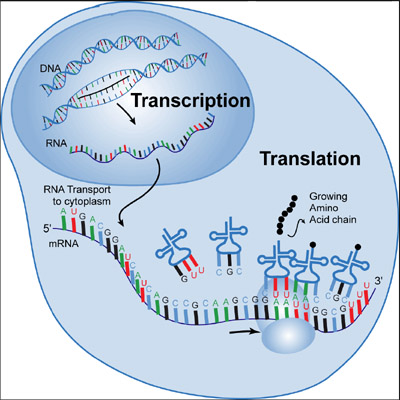
\includegraphics[height = 9cm, width = 9cm]{img/transcp_transla.jpg}
\caption{Transcription and Translation. From:  \href{http://www.tokresource.org}{tokresource.org}\label{fig:trans_trans}}
\end{center}
\end{figure}

\begin{figure}[!h]
\begin{center}
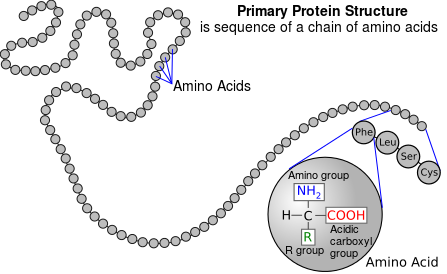
\includegraphics[ width = 8cm]{img/pro_amin.jpg}
\caption{Protein sequence. (From:  \href{http://www.wikimedia.org/}{wikimedia.org}) \label{fig:pro_se}}
\end{center}
\end{figure}

\section{Protein}
\textcolor{red}{add 1,2,3,4 structure of proteins}
Proteins are made of twenty kinds of amino acids. The function of proteins varies. The main functions of proteins can be working as antibodies, contractile proteins, enzymes, hormonal proteins, structural, storage proteins, transport proteins, etc. (\cite{white1959principles}).
In bioinformatics, we usually use FASTA format files to represent the amino acid sequences of proteins in an organism.
A FASTA file consists of protein or DNA names, description and sequences. Identifiers are preceded by a greater-than symbol "\textgreater" and the rest of the line is a description (optional). The next lines up to the next greater-than symbol contain the actual DNA or protein sequence. Figure \ref{fig:fasta} shows an example of a FASTA format. The protein name "YPR161C" follows the "\textgreater" sign. The protein sequence is given in the next five lines.


\begin{figure}
\begin{center}
\ttfamily{

	\begin{tabular}{p{2pt}p{2pt}p{2pt}p{2pt}p{2pt}p{2pt}p{2pt}p{2pt}p{2pt}p{2pt}p{2pt}p{2pt}p{2pt}p{2pt}p{2pt}p{2pt}p{2pt}p{2pt}p{2pt}p{2pt}p{2pt}p{2pt}p{2pt}p{2pt}p{2pt}p{2pt}p{2pt}}
	> & Y & P & R & 1 & 6 & 1 & C & \\ 
	T & T & G & A & C & M & T & T & G & A & C & M &T & T & G & A & C & M &V & V & V & R & N & M &\\ 
	 A & C & M &T & T & G & A & C&T & T & G & A & C & M & T & T & G  & M &T & T & G & A & C & M &\\ 
	Q & S & D& A & V & M & T & T & G & A & C & M &T & T & G & A & C & M &T & T & G & A & C & M &\\ 
	A & C & M &T & T & G & A & C & M & T & T & G & A & C & M &T & T & G & T & T & G & A & C & M &\\ 
	T & T & G & A & C & M & T & T & G & A & C & M &T & T &\\ 
	\end{tabular} \\

}
\caption{A protein in FASTA format.\label{fig:fasta}}
\end{center}
\end{figure}
\section{Protein-protein Interaction}
Proteins are some of the most important molecules in cells (\cite{schleif1993genetics}). 
They carry out most of the cellular processes. Quite often, they keep the cells functioning by interacting with other proteins in stable or transient protein complexes (\cite{eisenberg2000protein}).
This process is called protein-protein interaction (PPI). This is a vital process because of the accepted idea that PPIs are responsible for cell's behaviour under different stimuli (\cite{bader2003functional, pandey2000proteomics, schwikowski2000network}).
Protein complexes are groups of proteins that interact together to perform certain functions. Figure \ref{fig:pro_comp} shows an example of a protein complex. Protein pathways and modules are another two functional groups connected through PPIs. 
\begin{figure}[h!]
\begin{center}
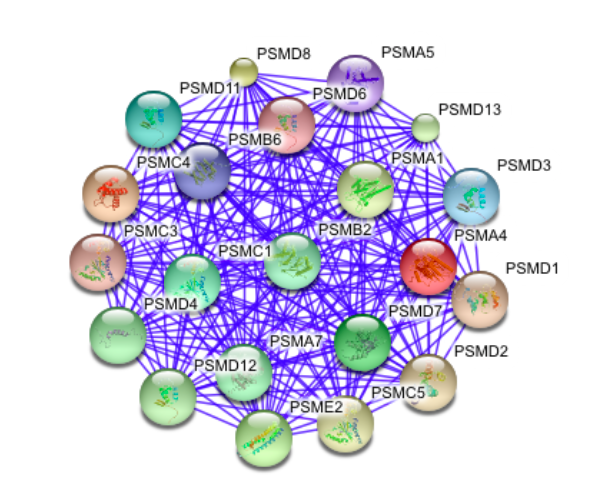
\includegraphics[height = 8cm]{img/pro_comp.png}
\caption{Protein complex. (From: bioproximity.com)  \label{fig:pro_comp}}
\end{center}
\end{figure}
 Scientists believe the reason that advanced organisms like humans are more complicated than lower organisms like the worms is not only because of large number of genes, but also because of sophisticated PPI networks \cite{pitre2008computational}. Figure \ref{fig:ppi_net} shows a map of human PPIs.
Understanding the potential of unknown proteins is becoming possible by looking into their PPI information \cite{sharan2007network}. As well, knowing PPI information helps improve the system-level understanding of molecular processes \cite{levy2008evolution}.
Therefore, understanding and mapping PPIs is an important current area of research.

\begin{figure}[h!]
\begin{center}
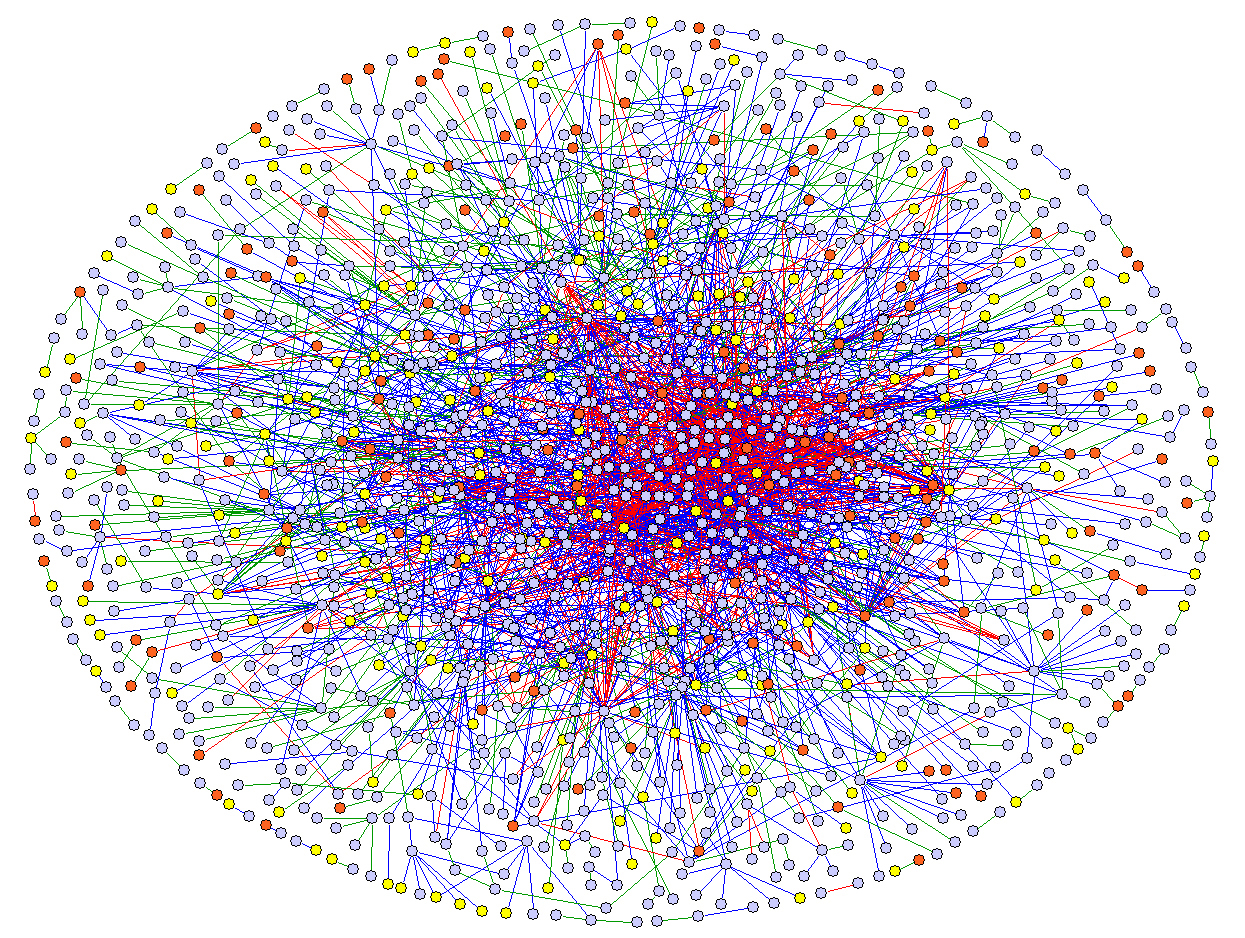
\includegraphics[height = 10cm, width = 10cm]{img/pro_inter_net.jpg}
\caption{A human protein-protein interaction network. (From: \href{https://www.mdc-berlin.de/}{www.mdc-berlin.de})  \label{fig:ppi_net}}
\end{center}
\end{figure}

However, there are a lot of unknown facts about PPIs to be discovered. For example, in a simple organism such as Saccharomyces cerevisiae, there are less than 40,000 estimated PPIs. Comparing with 19,000,000 potential interacting pair, it is believed that there is still a significant gap between known PPIs and real ones \cite{jessulat2011recent, sprinzak2003reliable}. Precise, fast and affordable protein-protein interaction prediction methods are needed.

The idea of PPI prediction is shown in Figure \ref{fig:ppi_pred}. The left part contains fours proteins and two known interactions, indicated using circles and blue lines respectively. Using those as inputs, PPI prediction methods would output a predicted interaction, indicated by the red line in the right picture. 
\begin{figure}[h!]
\begin{center}
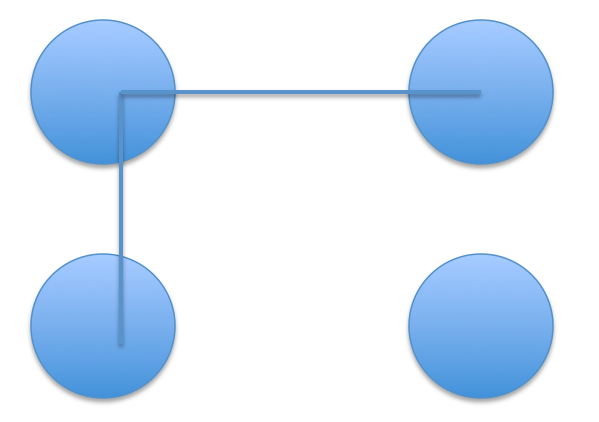
\includegraphics[width=6cm]{img/know_ppi.png}
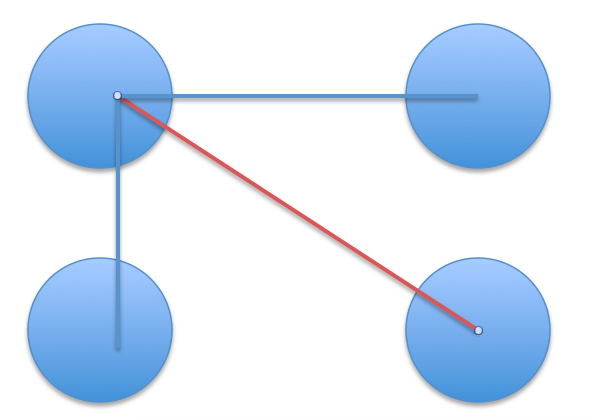
\includegraphics[width=6cm]{img/predict_ppi.png}
\end{center}
\caption{The idea of protein-protein interaction prediction.  \label{fig:ppi_pred}}
\end{figure}

There are many proposed PPI prediction methods, both experimental and computational ones. The most widely used experimental methods are Yeast two-hybrid (Y2H) \cite{fields1989novel} and Tandem affinity purification (TAP) \cite{suter2008two}. 

The yeast two-hybrid (Y2H) detects a protein interaction by telling the signal generated by the DNA-binding domain (DBD) and the activation domain (AD). There are several drawbacks of this approach. First, it can only detect PPIs within the nucleus. Second, it can only detect one interaction at a time, which is quite inefficient. Also, the false positive and false negative rates are high \cite{stephens2000use, semple2002jury}.

Tandem affinity purification (TAP) detects protein interactions by attaching a tag to the protein complex. After tagging, the complex is washed twice to remove the tag and unstable bindings. Isolated interacting proteins can be found if there are some. After washing, the mass spectrometry or other methods will be used to detect remaining proteins. The remaining ones are marked as interacting proteins \cite{rigaut1999generic}. A major advantage of the TAP approach is that it can detect interactions of protein complexes (more than two proteins), even without the interacting pattern. However, the "tag" added to proteins is itself a disadvantage. It might become a confounding factor in a way that changes the interacting process. Also, some real interactions can be washed away during two times of washing, thus increasing the false negative rate \cite{jessulat2011recent}.

 The experimental approaches are generally time and labour consuming. Also, they have the limitation of being unable to detect some protein complexes. In addition, the false positive rate and false negative rate of those approaches are high (\cite{pitre2006pipe}). Due to these disadvantages, computational approaches are proposed. Currently, there are mainly six kinds of computational PPI prediction approaches: genomic approach, evolutionary relationship approach, protein structure approach, domain approach, network analysis approach, and primary protein structure approach \cite{jessulat2011recent}. Our focus will be on the primary protein structure, or sequence based, approaches, and we give more details in the next chapter.
 
\section{Protein-protein Interaction Binding Sites}
Proteins interact with each other by binding together. Figure \ref{fig:ppi_bind} shows two binding proteins. The connecting parts between the blue protein and the red protein are the two binding sites of this interaction. These binding sites/ sub-sequences mediate this interaction.
\begin{figure}[h!]
\begin{center}
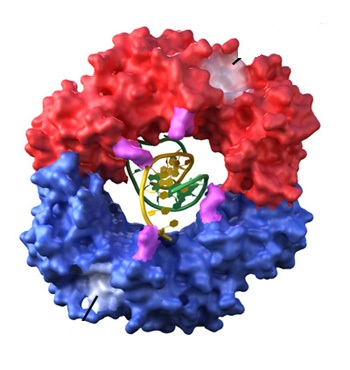
\includegraphics[width=6cm]{img/binding_sites.jpg}
\end{center}
\caption{Protein-protein interaction binding sites. (From: http://pdbj.org/eprots/) \label{fig:ppi_bind}}
\end{figure}

Knowing the binding sites help scientists understand cellular pathways better. However, the current protein interface predictors need improvements. Experimental approaches often report wrong binding
sites because of the wet lab processes, while computational approaches often require data which is not available at the proteome scale. \cite{amos2011binding}.

\begin{figure}[ht]
\begin{center}
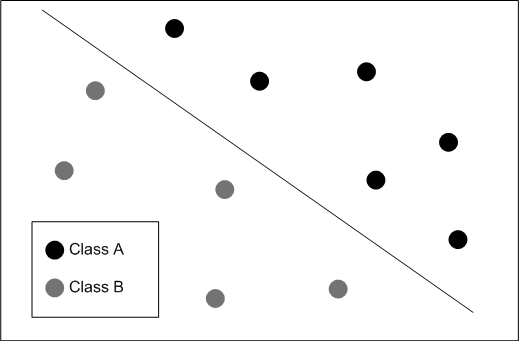
\includegraphics[height = 9cm, width = 9cm]{img/linear-classifier.png}
\caption{A long memory time series\label{ts1}}
\end{center}
\end{figure}

% Here's a table.
% \begin{table}[ht]
% \begin{center}
% \begin{tabular}[ht]{|c|lr|c|} 
%c stands for centre, l for left, r for right; the | puts lines in between, and the hline puts a horizontal line in
% \hline
% $n$ & $\alpha$ &$n\alpha$ & $\beta$\\
% \hline
% 1 & 0.2 & 0.2 & 5\\
% \hline
% 2 & 0.3 & 0.6 & 4\\
% \hline
% 3 & 0.7 & 2.1 & 3\\
% \hline
% \end{tabular}
% \caption{A random table \label{tab1}}
% \end{center}
% \end{table}

% \begin{eqnarray}
% y &=& mx + b \label{eq1}\\
% &=& ax+ c
% \label{eq2}
% \end{eqnarray}

% This is an un-numbered equation, along with a numbered one. 
% \begin{eqnarray}
% u &=& px \nonumber\\
% p &=& P(X=x) \label{eqn3}
% \end{eqnarray}

% Look at Table \ref{tab1} and Figure \ref{ts1} and equations \ref{eq1},  \ref{eq2}, and \ref{eqn3}.

% Let's do some matrix algebra now.

% \begin{equation}
% det\left(\left|\begin{array}{ccc} 2 & 3 & 5\\
% 4 & 4 & 6\\
% 9 & 8 & 1
% \end{array}\right|\right) = 42
% \end{equation}

% In the equation and eqnarray environments, you don't need to have the dollar sign to enter math mode.

% \begin{eqnarray}
% \alpha = \beta_1 \Gamma^{-1}
% \end{eqnarray}

% This is citing a reference ~\cite{zhang2019scriber}.  This is citing another ~\cite{zhang2019scriber}.  Nobody said something ~\cite{zhang2019scriber}.
